% The tower of fixed fields K ⊇ K^I ⊇ K^D ⊇ ℚ matched with the
% subgroup chain {1} ⊆ I ⊆ D ⊆ G, with the ramify/inert/split steps
% of sizes e, f, g.
% Source: book/tex/alg-NT/ramification.tex (§ (Optional)
% Decomposition and inertia groups) — tikzcd.
\documentclass[border=2mm]{standalone}
\usepackage{tikz}
\usetikzlibrary{arrows.meta}
\usepackage{amssymb}
\begin{document}
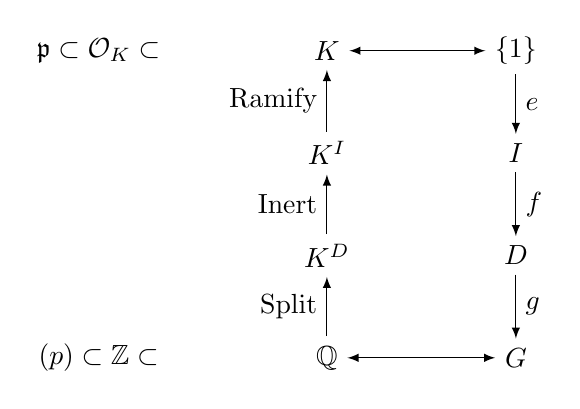
\begin{tikzpicture}[>=latex]
  \node (pK) at (-2.9,3.9) {$\mathfrak{p} \subset \mathcal{O}_K \subset$};
  \node (K) at (0,3.9) {$K$};
  \node (KI) at (0,2.6) {$K^I$};
  \node (KD) at (0,1.3) {$K^D$};
  \node (pQ) at (-2.9,0) {$(p) \subset \mathbb{Z} \subset$};
  \node (Q) at (0,0) {$\mathbb{Q}$};
  \node (e1) at (2.4,3.9) {$\{1\}$};
  \node (I) at (2.4,2.6) {$I$};
  \node (D) at (2.4,1.3) {$D$};
  \node (G) at (2.4,0) {$G$};
  \draw[<->] (K) -- (e1);
  \draw[<->] (Q) -- (G);
  \draw[->] (KI) -- (K) node[midway,left] {Ramify};
  \draw[->] (KD) -- (KI) node[midway,left] {Inert};
  \draw[->] (Q) -- (KD) node[midway,left] {Split};
  \draw[->] (e1) -- (I) node[midway,right] {$e$};
  \draw[->] (I) -- (D) node[midway,right] {$f$};
  \draw[->] (D) -- (G) node[midway,right] {$g$};
\end{tikzpicture}
\end{document}
